% !Mode:: "TeX:UTF-8"	% read in as utf8 file.

\chapter{Mesh Processing}

\section{Recsconstruct quad rib mesh}
See \lstinline[language=C++]|Run_reconstruct_quadRibMesh.cpp| and \lstinline[language=C++]|generalRibs3.cpp|
\begin{figure}[h!]
	\centering
	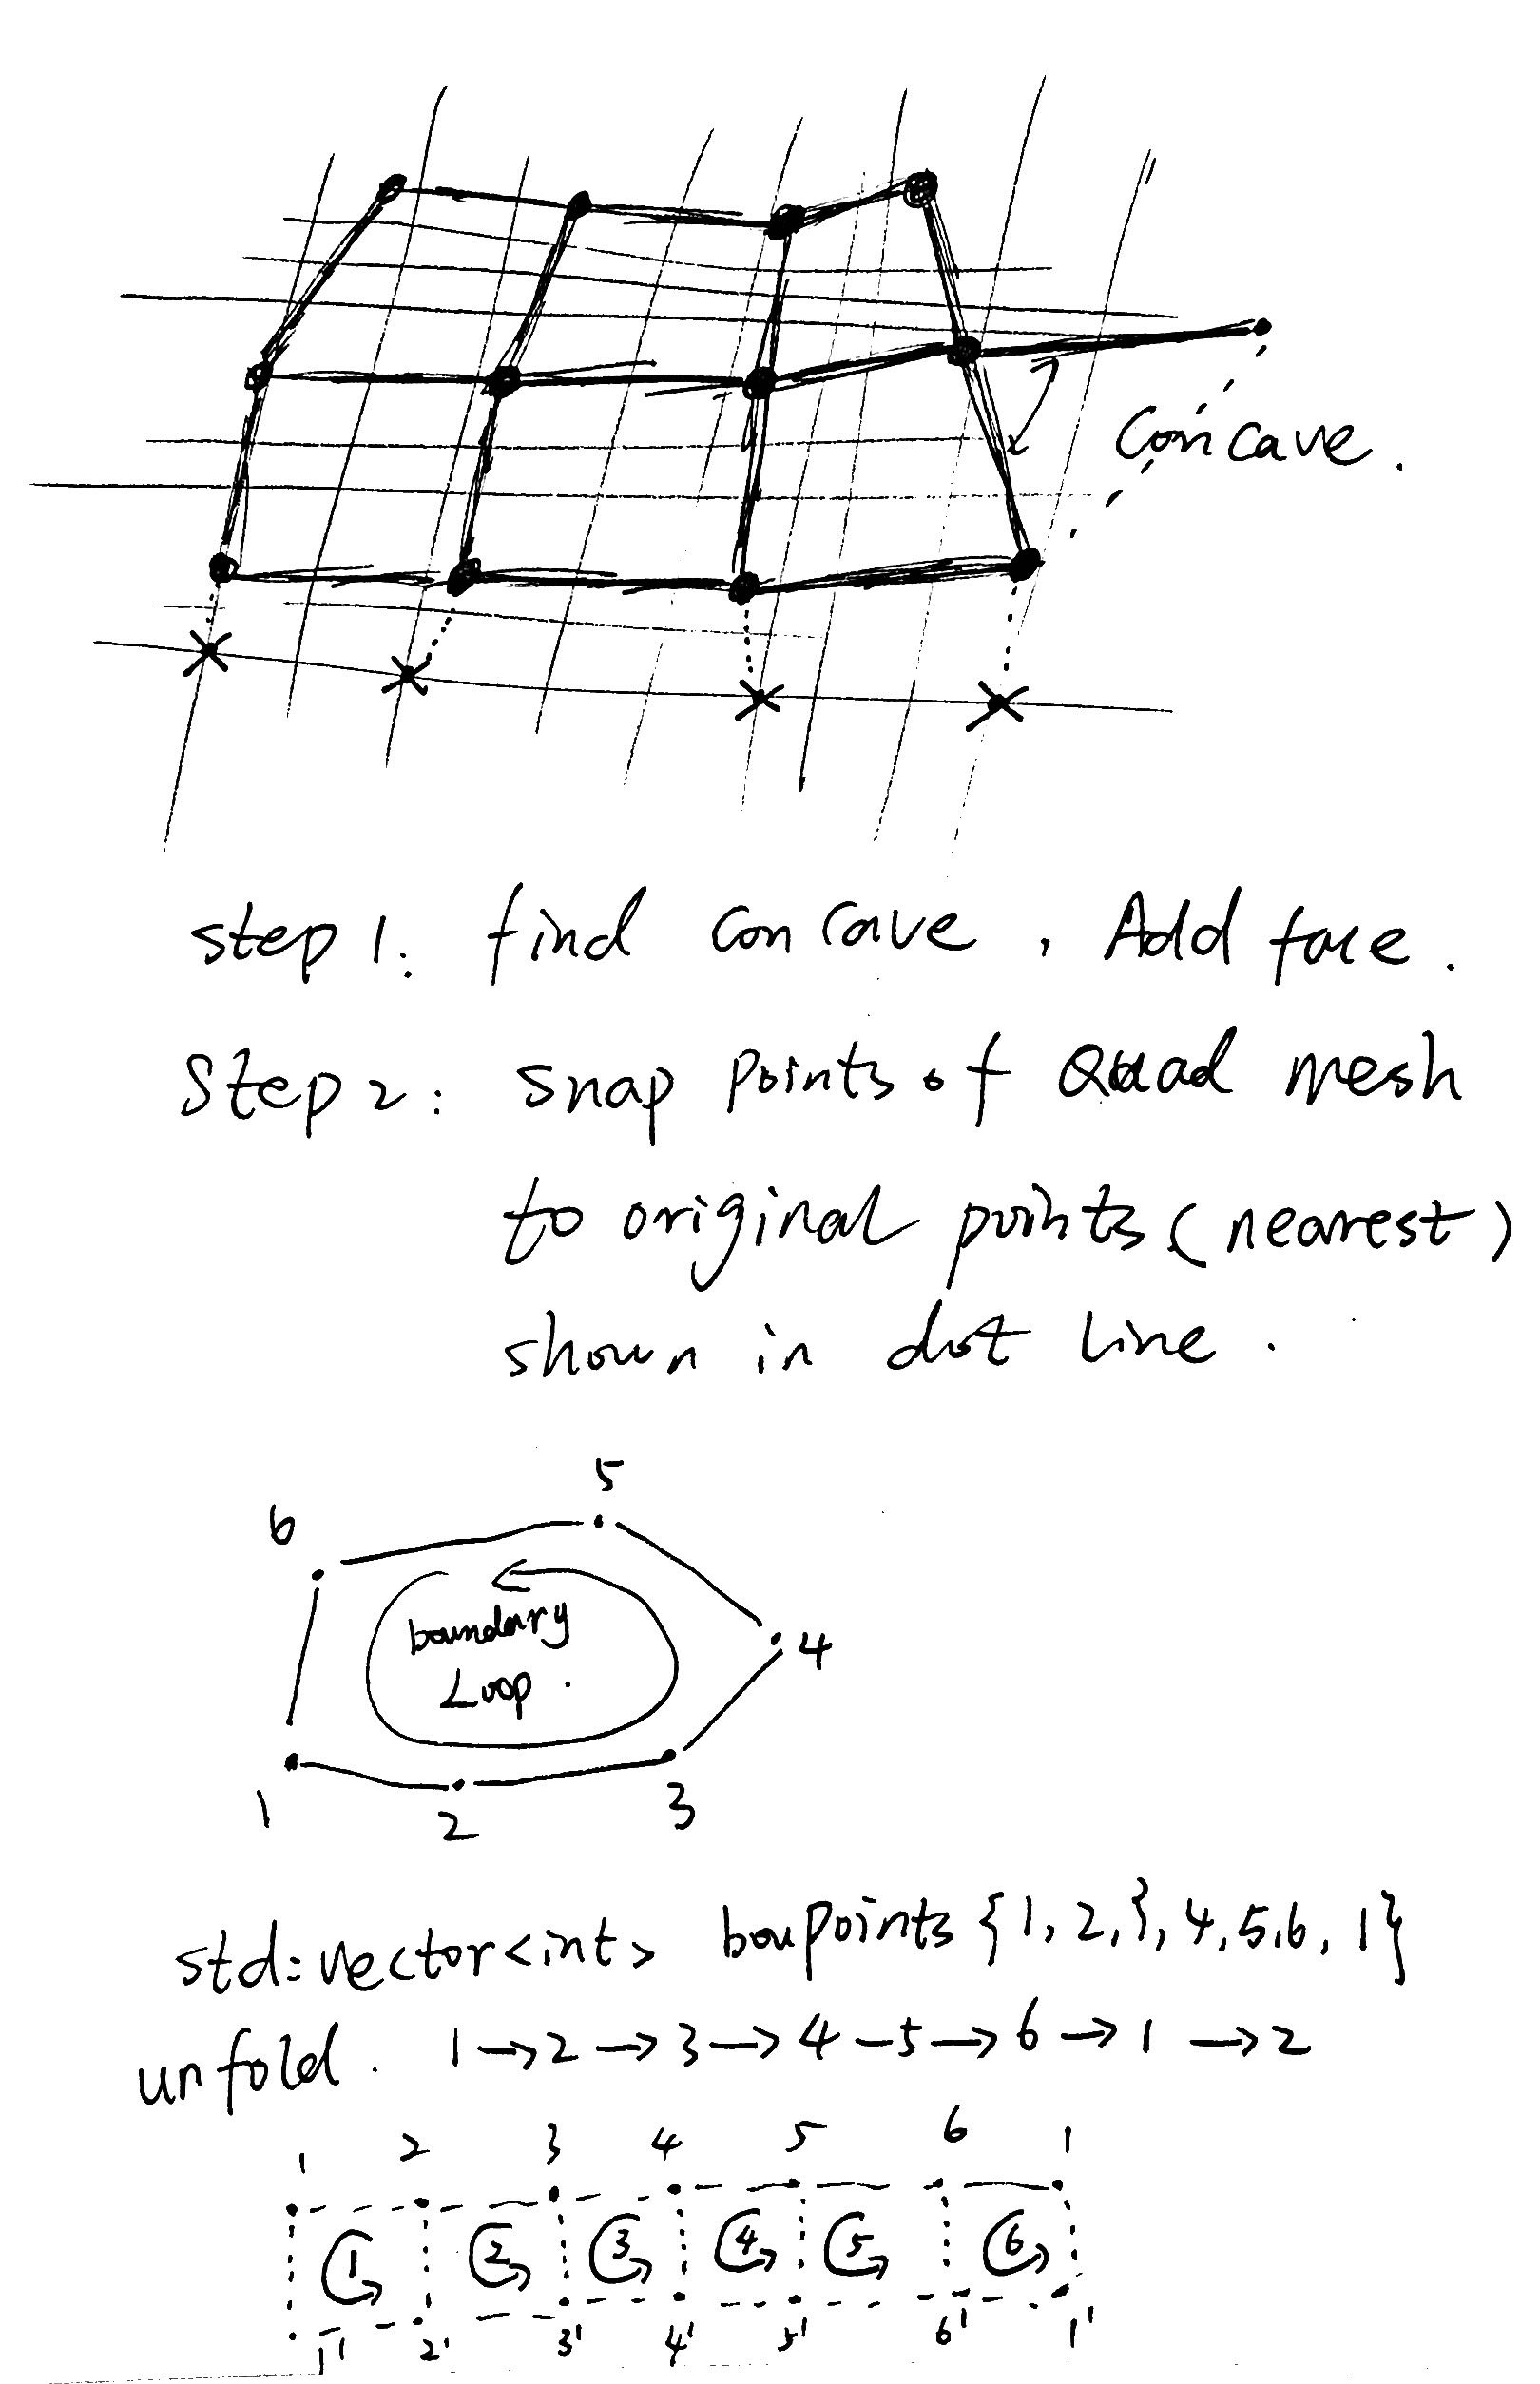
\includegraphics[width=0.7\linewidth]{Figures/reconstruct_quadRibMesh}
	\caption{reconstruct quad rib mesh}
	\label{fig:reconstructquadribmesh}
\end{figure}

\section{slice quad rib mesh}
See \lstinline[language=C++]|Run_slice_quadRibMesh.cpp| and \lstinline[language=C++]|generalRibs3.cpp|
\begin{figure}[h!]
	\centering
	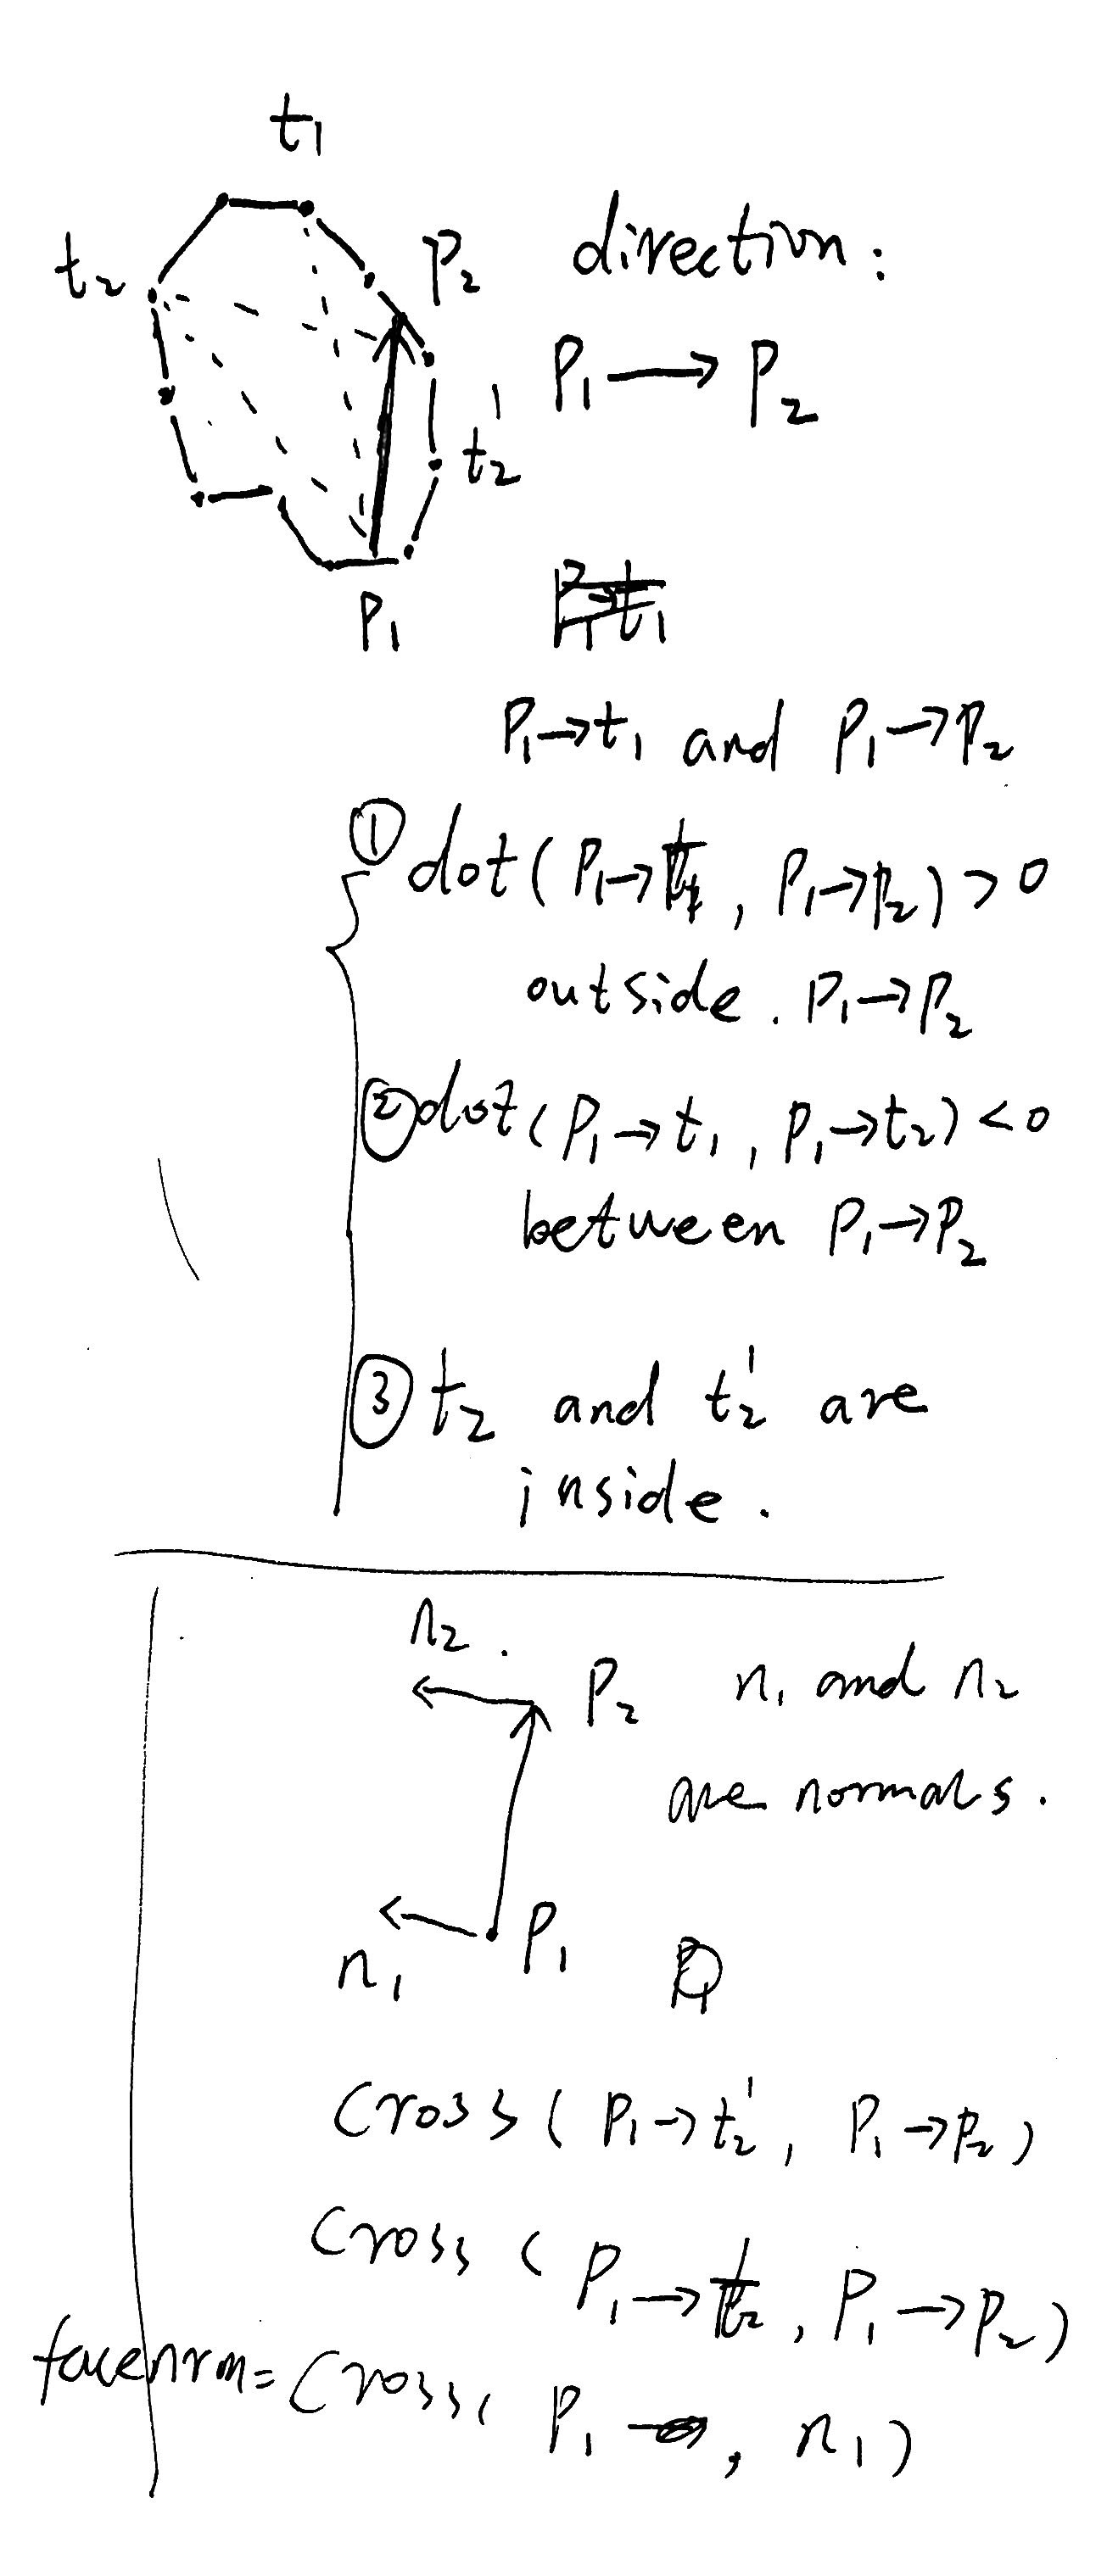
\includegraphics[width=0.7\linewidth]{Figures/slice_quadRibMesh}
	\caption{slice quad rib mesh}
	\label{fig:slicequadribmesh}
\end{figure}

\section{Laplacian Smoothing}
For each vertex in a mesh, a new position is chosed based on local information (such as the position of neighbors) and the veertex is moved there. In the case that a mesh is topologically a rectangular grid (that is, each internal vertex is connected to four neighbrs) then this operation produces the Laplacian of the mesh.

The smoothing operation may be described per-vertex as:

\begin{equation}
\bar{x}_i = \dfrac{1}{N} \sum_{j=1}^{N} \bar{x}_j
\end{equation}

Where $ N $ is the number of adjacent vertices to node $ i $, $ \bar{x}_j $ is the position of the $ j $-thadjacent vertex and $ \bar{x}_i $ is the new position for node $ i $

\section{Surface Parameterization}
A surface in 3-space can be parameterized by two variabls (or coordinates) $ u $ and $ v $ such that:

\begin{align}
	x &= x(u,v) \\
	y &= y(u,v) \\
	z &= z(u,v)
\end{align}

If a surface is parameterized as above, then the tangent vectors

\begin{align*}
	\mathbf{T}_u &= \dfrac{\partial x}{\partial u} \hat{\mathbf{x}} + \dfrac{\partial y}{\partial u} \hat{\mathbf{y}} + \dfrac{\partial z}{\partial u} \hat{\mathbf{z}} \\
	\mathbf{T}_v &= \dfrac{\partial x}{\partial v} \hat{\mathbf{x}} + \dfrac{\partial y}{\partial v} \hat{\mathbf{y}} + \dfrac{\partial z}{\partial v} \hat{\mathbf{z}}
\end{align*}


\section{Trace edges}

\section{Polyline to polygon}
Given a set of points arranged in anti-clockwise direction with thickness at each point, a polygon mesh is built based on these points.

The vertices enclosing the polygon are actually intersection vertices of two lines:

\begin{figure}[h!]
	\centering
	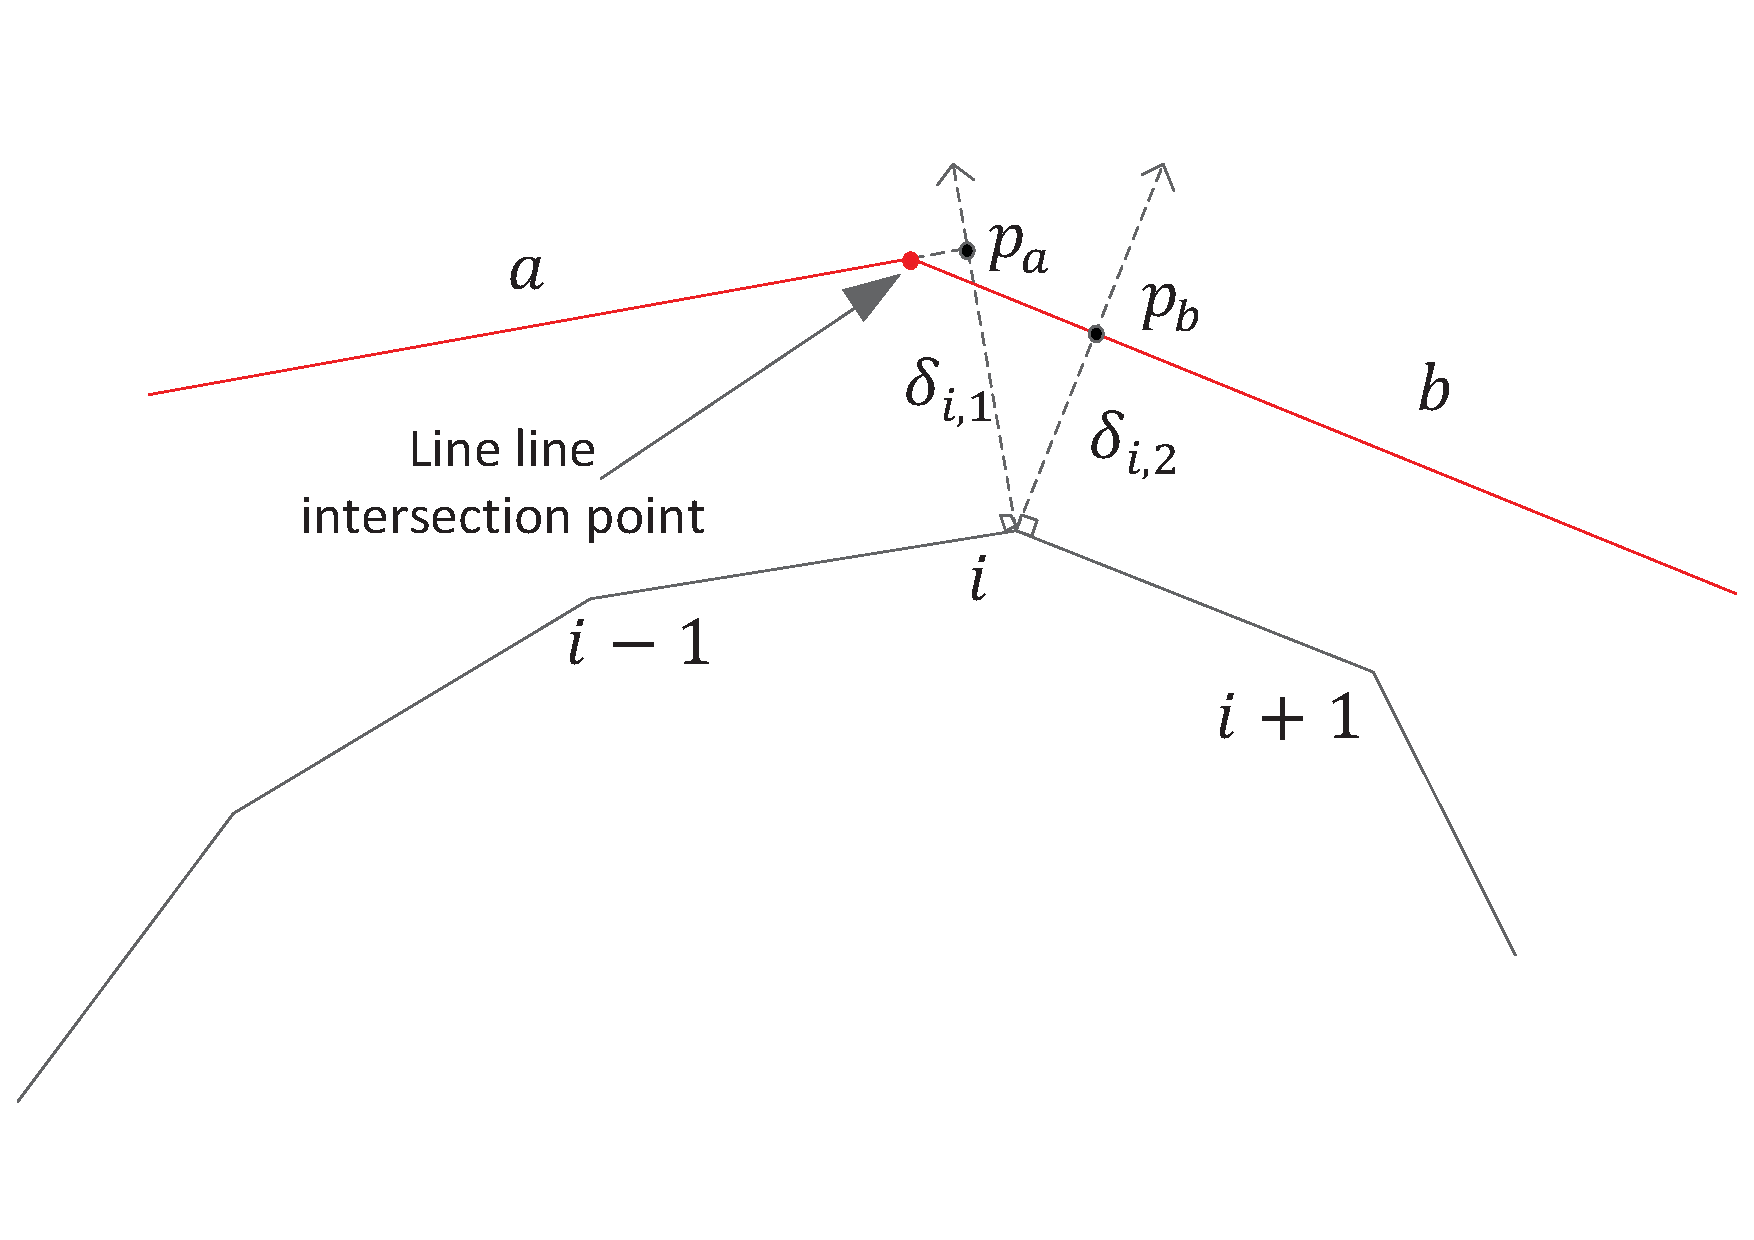
\includegraphics[width=0.5\linewidth]{Figures/polyline_intersectionPoint}
	\caption{Intersection points}
	\label{fig:polylineintersectionpoint}
\end{figure}

As can be seen in figure \ref{fig:polylineintersectionpoint}, $ p_a $ and $ p_b $ are two points above polylines with offse $ \delta_{i,1} $ and $ \delta_{i,2} $ separately. Two red lines $ a $ and $ b $ through $ p_a $ and $ p_b $  are built respectively.

The coordinates of $ p_a $ and $ p_b $ are:

\begin{align*}
p_a &= p_i + \frac{\delta_{i,1}}{2} \vec{e}_a \\
p_b &= p_i + \frac{\delta_{i,2}}{2} \vec{e}_b
\end{align*}

where $ \vec{e}_a = \mathrm{cross}([1;0;0], p_{i}-p_{i-1} ), \vec{e}_b = \mathrm{cross}([1;0;0], p_{i+1}-p_{i} )  $

and the equations for red lines are:
\begin{align*}
	\frac{z-z_a}{y-y_a} &= \frac{z_{i}-z_{i-1}}{y_{i}-y_{i-1}} \\
	\frac{z-z_b}{y-y_b} &= \frac{z_{i+1}-z_{i}}{y_{i+1}-y_{i}}
\end{align*}

The intersected point of two lines can be found by soling symbolic equations:

\begin{lstlisting}[language=matlab]
function SolveIntersectionPoint()
% syms y1 z1 y2 z2 y3 z3
syms t1 t2 t3 t4
syms ya za yb zb
syms y z

%  z-za     z2-z1     t1
% ------ = ------- = -----
%  y-ya     y2-y1     t2

%  z-zb     z3-z2     t3
% ------ = ------- = -----
%  y-yb     y3-y2     t4

% [y, z] = solve( (z-za)/(y-ya) == (z2-z1)/(y2-y1), (z-zb)/(y-yb) == (z3-z2)/(y3-y2), y, z );
[y, z] = solve( (z-za)/(y-ya) == t1/t2, (z-zb)/(y-yb) == t3/t4, y, z )

% results.
% y = (t1*t4*ya - t2*t3*yb - t2*t4*za + t2*t4*zb)/(t1*t4 - t2*t3)
% z = (t1*t3*ya - t1*t3*yb - t2*t3*za + t1*t4*zb)/(t1*t4 - t2*t3)

end % end of function.
\end{lstlisting}

After having all vertices for the polygon, the mesh is obtained in figure \ref{fig:polyline2polygon}:

\begin{figure}[h!]
\centering
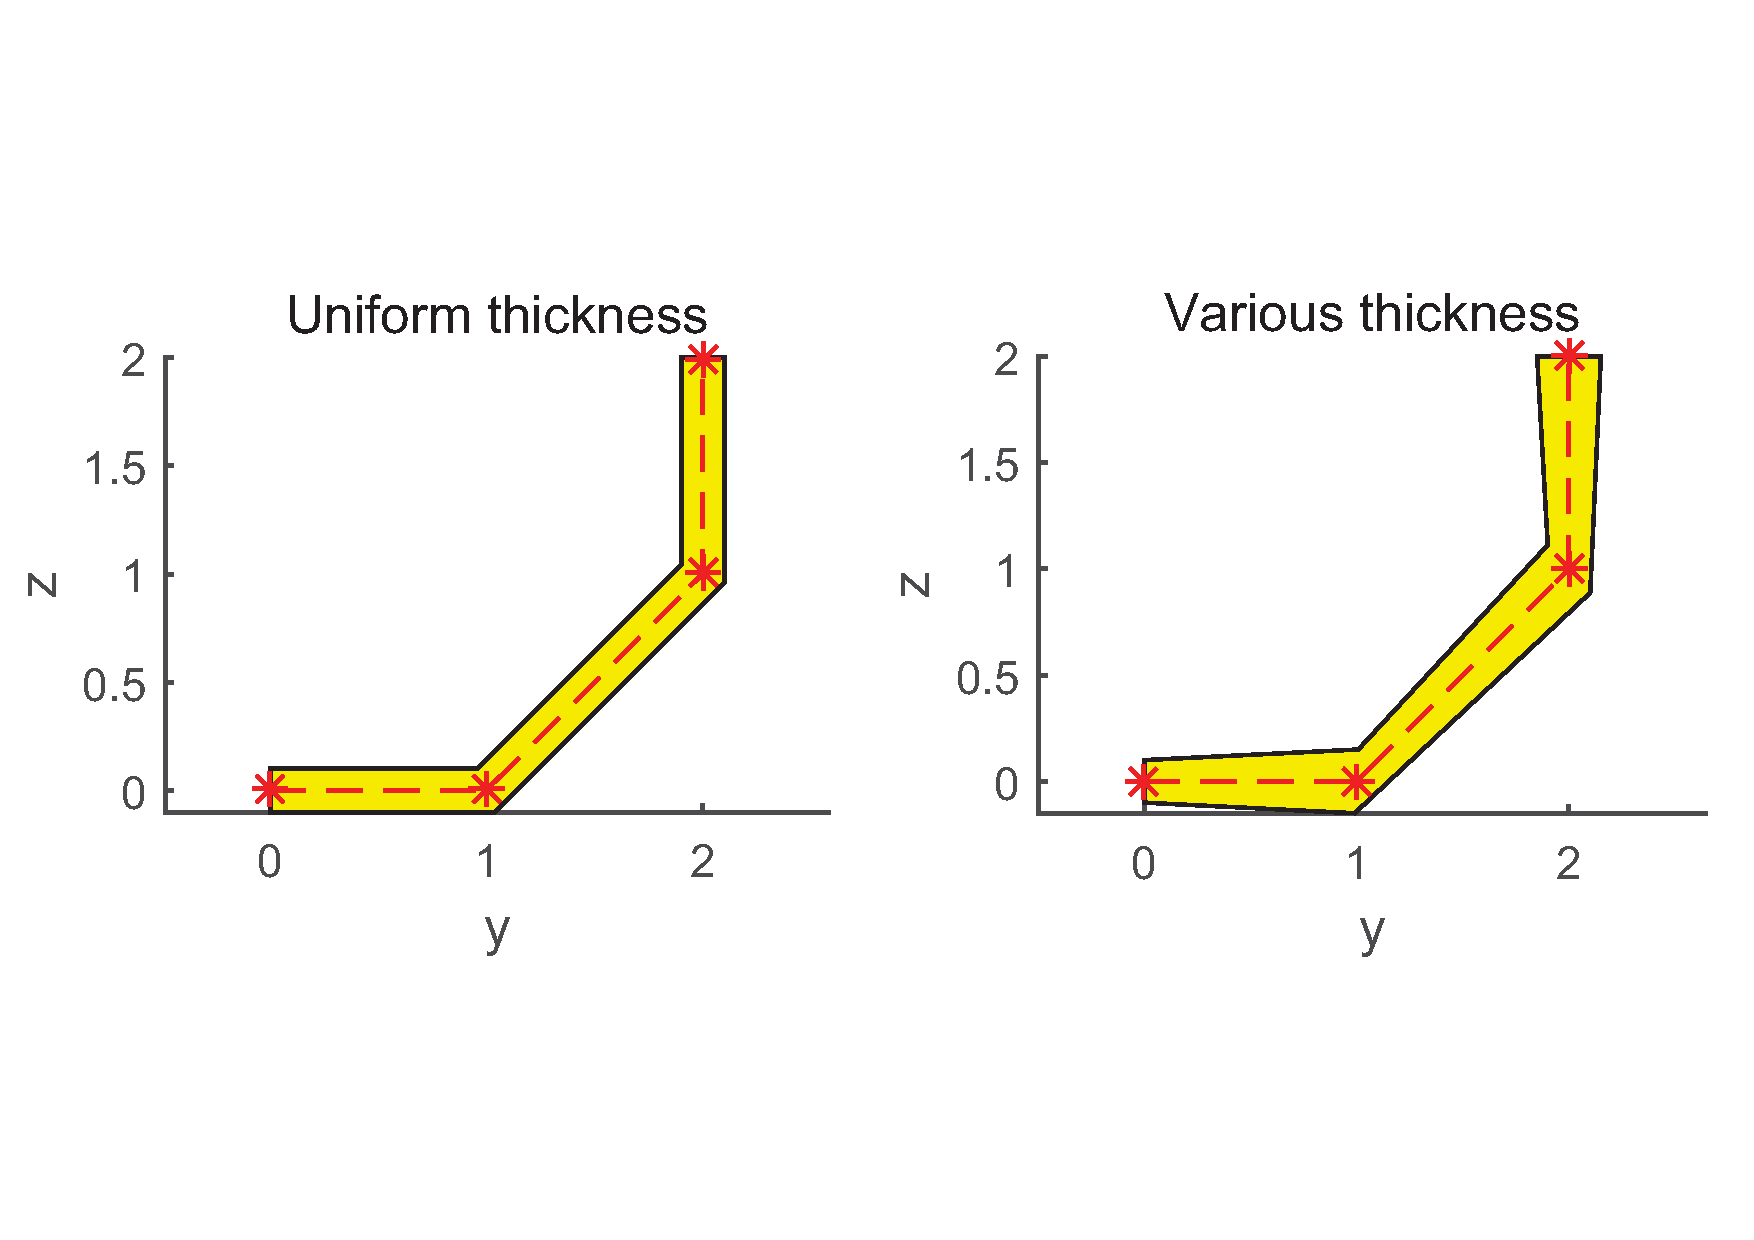
\includegraphics[width=0.7\linewidth]{Figures/polyline2Polygon}
\caption{polygon formed from polyline}
\label{fig:polyline2polygon}
\end{figure}

Note the red lines are the input polyline.